% Created by tikzDevice version 0.12.3 on 2019-08-31 17:49:46
% !TEX encoding = UTF-8 Unicode
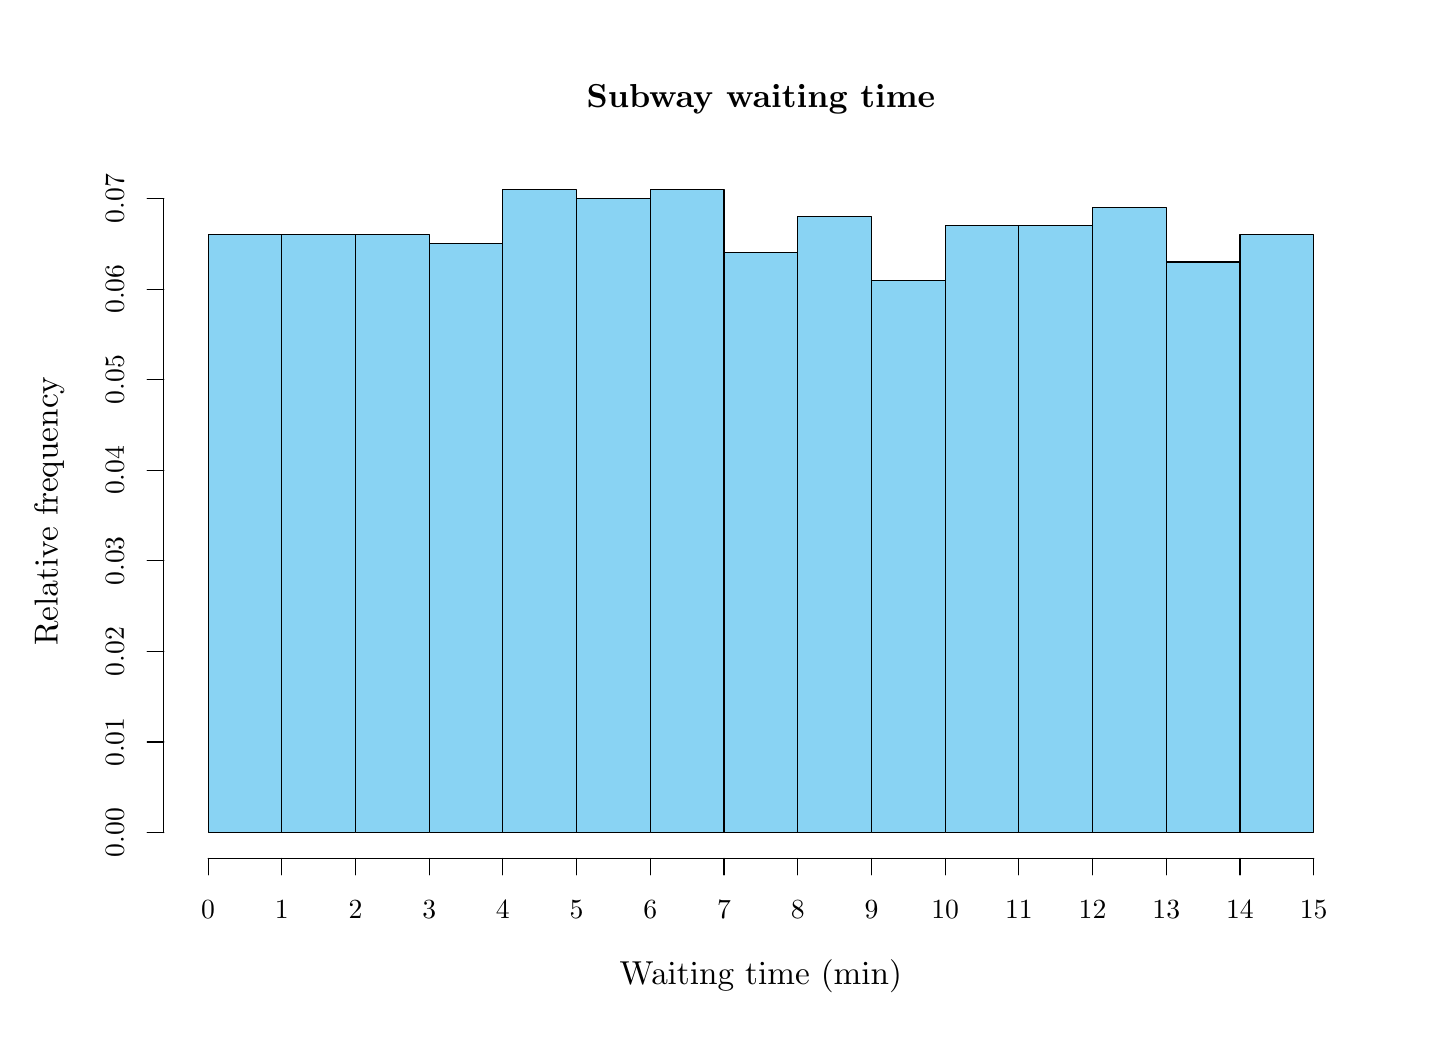
\begin{tikzpicture}[x=1pt,y=1pt]
\definecolor{fillColor}{RGB}{255,255,255}
\path[use as bounding box,fill=fillColor,fill opacity=0.00] (0,0) rectangle (505.89,361.35);
\begin{scope}
\path[clip] (  0.00,  0.00) rectangle (505.89,361.35);
\definecolor{drawColor}{RGB}{0,0,0}

\node[text=drawColor,anchor=base,inner sep=0pt, outer sep=0pt, scale=  1.20] at (264.94,332.61) {\bfseries Subway waiting time};

\node[text=drawColor,anchor=base,inner sep=0pt, outer sep=0pt, scale=  1.20] at (264.94, 15.60) {Waiting time (min)};

\node[text=drawColor,rotate= 90.00,anchor=base,inner sep=0pt, outer sep=0pt, scale=  1.20] at ( 10.80,186.67) {Relative frequency};
\end{scope}
\begin{scope}
\path[clip] (  0.00,  0.00) rectangle (505.89,361.35);
\definecolor{drawColor}{RGB}{0,0,0}

\path[draw=drawColor,line width= 0.4pt,line join=round,line cap=round] ( 49.20, 70.49) -- ( 49.20,299.58);

\path[draw=drawColor,line width= 0.4pt,line join=round,line cap=round] ( 49.20, 70.49) -- ( 43.20, 70.49);

\path[draw=drawColor,line width= 0.4pt,line join=round,line cap=round] ( 49.20,103.22) -- ( 43.20,103.22);

\path[draw=drawColor,line width= 0.4pt,line join=round,line cap=round] ( 49.20,135.95) -- ( 43.20,135.95);

\path[draw=drawColor,line width= 0.4pt,line join=round,line cap=round] ( 49.20,168.68) -- ( 43.20,168.68);

\path[draw=drawColor,line width= 0.4pt,line join=round,line cap=round] ( 49.20,201.40) -- ( 43.20,201.40);

\path[draw=drawColor,line width= 0.4pt,line join=round,line cap=round] ( 49.20,234.13) -- ( 43.20,234.13);

\path[draw=drawColor,line width= 0.4pt,line join=round,line cap=round] ( 49.20,266.86) -- ( 43.20,266.86);

\path[draw=drawColor,line width= 0.4pt,line join=round,line cap=round] ( 49.20,299.58) -- ( 43.20,299.58);

\node[text=drawColor,rotate= 90.00,anchor=base,inner sep=0pt, outer sep=0pt, scale=  1.00] at ( 34.80, 70.49) {0.00};

\node[text=drawColor,rotate= 90.00,anchor=base,inner sep=0pt, outer sep=0pt, scale=  1.00] at ( 34.80,103.22) {0.01};

\node[text=drawColor,rotate= 90.00,anchor=base,inner sep=0pt, outer sep=0pt, scale=  1.00] at ( 34.80,135.95) {0.02};

\node[text=drawColor,rotate= 90.00,anchor=base,inner sep=0pt, outer sep=0pt, scale=  1.00] at ( 34.80,168.68) {0.03};

\node[text=drawColor,rotate= 90.00,anchor=base,inner sep=0pt, outer sep=0pt, scale=  1.00] at ( 34.80,201.40) {0.04};

\node[text=drawColor,rotate= 90.00,anchor=base,inner sep=0pt, outer sep=0pt, scale=  1.00] at ( 34.80,234.13) {0.05};

\node[text=drawColor,rotate= 90.00,anchor=base,inner sep=0pt, outer sep=0pt, scale=  1.00] at ( 34.80,266.86) {0.06};

\node[text=drawColor,rotate= 90.00,anchor=base,inner sep=0pt, outer sep=0pt, scale=  1.00] at ( 34.80,299.58) {0.07};
\end{scope}
\begin{scope}
\path[clip] ( 49.20, 61.20) rectangle (480.69,312.15);
\definecolor{drawColor}{RGB}{0,0,0}
\definecolor{fillColor}{RGB}{137,211,243}

\path[draw=drawColor,line width= 0.4pt,line join=round,line cap=round,fill=fillColor] ( 65.18, 70.49) rectangle ( 91.82,286.49);

\path[draw=drawColor,line width= 0.4pt,line join=round,line cap=round,fill=fillColor] ( 91.82, 70.49) rectangle (118.45,286.49);

\path[draw=drawColor,line width= 0.4pt,line join=round,line cap=round,fill=fillColor] (118.45, 70.49) rectangle (145.09,286.49);

\path[draw=drawColor,line width= 0.4pt,line join=round,line cap=round,fill=fillColor] (145.09, 70.49) rectangle (171.72,283.22);

\path[draw=drawColor,line width= 0.4pt,line join=round,line cap=round,fill=fillColor] (171.72, 70.49) rectangle (198.36,302.86);

\path[draw=drawColor,line width= 0.4pt,line join=round,line cap=round,fill=fillColor] (198.36, 70.49) rectangle (224.99,299.58);

\path[draw=drawColor,line width= 0.4pt,line join=round,line cap=round,fill=fillColor] (224.99, 70.49) rectangle (251.63,302.86);

\path[draw=drawColor,line width= 0.4pt,line join=round,line cap=round,fill=fillColor] (251.63, 70.49) rectangle (278.26,279.95);

\path[draw=drawColor,line width= 0.4pt,line join=round,line cap=round,fill=fillColor] (278.26, 70.49) rectangle (304.90,293.04);

\path[draw=drawColor,line width= 0.4pt,line join=round,line cap=round,fill=fillColor] (304.90, 70.49) rectangle (331.53,270.13);

\path[draw=drawColor,line width= 0.4pt,line join=round,line cap=round,fill=fillColor] (331.53, 70.49) rectangle (358.17,289.76);

\path[draw=drawColor,line width= 0.4pt,line join=round,line cap=round,fill=fillColor] (358.17, 70.49) rectangle (384.80,289.76);

\path[draw=drawColor,line width= 0.4pt,line join=round,line cap=round,fill=fillColor] (384.80, 70.49) rectangle (411.44,296.31);

\path[draw=drawColor,line width= 0.4pt,line join=round,line cap=round,fill=fillColor] (411.44, 70.49) rectangle (438.07,276.67);

\path[draw=drawColor,line width= 0.4pt,line join=round,line cap=round,fill=fillColor] (438.07, 70.49) rectangle (464.71,286.49);
\end{scope}
\begin{scope}
\path[clip] (  0.00,  0.00) rectangle (505.89,361.35);
\definecolor{drawColor}{RGB}{0,0,0}

\path[draw=drawColor,line width= 0.4pt,line join=round,line cap=round] ( 65.18, 61.20) -- (464.71, 61.20);

\path[draw=drawColor,line width= 0.4pt,line join=round,line cap=round] ( 65.18, 61.20) -- ( 65.18, 55.20);

\path[draw=drawColor,line width= 0.4pt,line join=round,line cap=round] ( 91.82, 61.20) -- ( 91.82, 55.20);

\path[draw=drawColor,line width= 0.4pt,line join=round,line cap=round] (118.45, 61.20) -- (118.45, 55.20);

\path[draw=drawColor,line width= 0.4pt,line join=round,line cap=round] (145.09, 61.20) -- (145.09, 55.20);

\path[draw=drawColor,line width= 0.4pt,line join=round,line cap=round] (171.72, 61.20) -- (171.72, 55.20);

\path[draw=drawColor,line width= 0.4pt,line join=round,line cap=round] (198.36, 61.20) -- (198.36, 55.20);

\path[draw=drawColor,line width= 0.4pt,line join=round,line cap=round] (224.99, 61.20) -- (224.99, 55.20);

\path[draw=drawColor,line width= 0.4pt,line join=round,line cap=round] (251.63, 61.20) -- (251.63, 55.20);

\path[draw=drawColor,line width= 0.4pt,line join=round,line cap=round] (278.26, 61.20) -- (278.26, 55.20);

\path[draw=drawColor,line width= 0.4pt,line join=round,line cap=round] (304.90, 61.20) -- (304.90, 55.20);

\path[draw=drawColor,line width= 0.4pt,line join=round,line cap=round] (331.53, 61.20) -- (331.53, 55.20);

\path[draw=drawColor,line width= 0.4pt,line join=round,line cap=round] (358.17, 61.20) -- (358.17, 55.20);

\path[draw=drawColor,line width= 0.4pt,line join=round,line cap=round] (384.80, 61.20) -- (384.80, 55.20);

\path[draw=drawColor,line width= 0.4pt,line join=round,line cap=round] (411.44, 61.20) -- (411.44, 55.20);

\path[draw=drawColor,line width= 0.4pt,line join=round,line cap=round] (438.07, 61.20) -- (438.07, 55.20);

\path[draw=drawColor,line width= 0.4pt,line join=round,line cap=round] (464.71, 61.20) -- (464.71, 55.20);

\node[text=drawColor,anchor=base,inner sep=0pt, outer sep=0pt, scale=  1.00] at ( 65.18, 39.60) {0};

\node[text=drawColor,anchor=base,inner sep=0pt, outer sep=0pt, scale=  1.00] at ( 91.82, 39.60) {1};

\node[text=drawColor,anchor=base,inner sep=0pt, outer sep=0pt, scale=  1.00] at (118.45, 39.60) {2};

\node[text=drawColor,anchor=base,inner sep=0pt, outer sep=0pt, scale=  1.00] at (145.09, 39.60) {3};

\node[text=drawColor,anchor=base,inner sep=0pt, outer sep=0pt, scale=  1.00] at (171.72, 39.60) {4};

\node[text=drawColor,anchor=base,inner sep=0pt, outer sep=0pt, scale=  1.00] at (198.36, 39.60) {5};

\node[text=drawColor,anchor=base,inner sep=0pt, outer sep=0pt, scale=  1.00] at (224.99, 39.60) {6};

\node[text=drawColor,anchor=base,inner sep=0pt, outer sep=0pt, scale=  1.00] at (251.63, 39.60) {7};

\node[text=drawColor,anchor=base,inner sep=0pt, outer sep=0pt, scale=  1.00] at (278.26, 39.60) {8};

\node[text=drawColor,anchor=base,inner sep=0pt, outer sep=0pt, scale=  1.00] at (304.90, 39.60) {9};

\node[text=drawColor,anchor=base,inner sep=0pt, outer sep=0pt, scale=  1.00] at (331.53, 39.60) {10};

\node[text=drawColor,anchor=base,inner sep=0pt, outer sep=0pt, scale=  1.00] at (358.17, 39.60) {11};

\node[text=drawColor,anchor=base,inner sep=0pt, outer sep=0pt, scale=  1.00] at (384.80, 39.60) {12};

\node[text=drawColor,anchor=base,inner sep=0pt, outer sep=0pt, scale=  1.00] at (411.44, 39.60) {13};

\node[text=drawColor,anchor=base,inner sep=0pt, outer sep=0pt, scale=  1.00] at (438.07, 39.60) {14};

\node[text=drawColor,anchor=base,inner sep=0pt, outer sep=0pt, scale=  1.00] at (464.71, 39.60) {15};
\end{scope}
\end{tikzpicture}
